\documentclass[12pt]{article}
\usepackage[a4paper, left=3.17cm, right=3.17cm, top=2.54cm, bottom=2.54cm]{geometry}
\usepackage[UTF8]{ctex}
\usepackage{newtxtext,newtxmath} % Use Times font
\usepackage{amsmath}
\usepackage{amsfonts}
\usepackage{chemformula}
\usepackage{cite}
\usepackage[colorlinks, linkcolor=black, anchorcolor=black, citecolor=black]{hyperref}
\usepackage{graphicx}
\usepackage{subfigure}
\usepackage{makecell}
\usepackage{caption}
\usepackage{booktabs}
\usepackage{abstract}
\usepackage{longtable}
\usepackage{float}

\renewcommand{\abstractname}{\Large\textbf{摘要}}

\setlength{\parskip}{0.5em}
\title{线性V/F转换}
\author{\textup{廖章盛}}
\begin{document}

\begin{titlepage}
\setcounter{page}{0}
    \newcommand{\HRule}{\rule{\linewidth}{0.5mm}}
    \centering
    
\includegraphics[width=8cm]{fig/DHU.png}\\[1cm]
    \quad\\[1.5cm]
    \textsl{\Large 东华大学 }\\[0.5cm]
    \textsl{\large 课程设计报告}\\[0.5cm]

    \makeatletter
    \HRule \\[0.4cm]
    { \huge \bfseries \@title}\\[0.4cm]
    \HRule \\[1.5cm]
    {\large
    \begin{tabular}{c@{~~}c}
        \makebox[2em][s]{专业}: & \underline{\makebox[8em][c]{自动化2102}} \\
        \makebox[2em][s]{姓名}: & \underline{\makebox[8em][c]{廖章盛}}     \\
        \makebox[2em][s]{学号}: & \underline{\makebox[8em][c]{211140215}}  \\
        \makebox[2em][s]{批次}: & \underline{\makebox[8em][c]{B班 50号}}  \\
    \end{tabular}\\[1cm]}
    \makeatother
    {\large \today}\\[2cm]
    \vfill
\end{titlepage}

\begin{abstract}
电压频率转换器VFC(Voltage Frequency Converter)是一种实现模数转换功能的器件,将模拟电压量转换为脉冲信号,使得输出脉冲信号的频率与输出电压大小成正比。V/F转换电路的应用十分广泛,学习这个电路对于提升模拟电子技术的理解很有帮助。本报告介绍了一种利用集成运算放大器、555单稳态触发器和三极管模拟控制开关搭建的线性 V/F 转换器,实现了输入电压与输出频率的线性变换。

本报告首先对线性 V/F 转换器的原理及电路框图进行了详细分析,包括输入信号、阻抗变换、基准源、积分电路、脉冲输出电路和开关电路等各个模块的功能和电路图。

计算机软件仿真部分,利用 multisim 仿真软件进行了电路设计和原理仿真,选取了合适的原件参数,并通过示波器观察了输出波形,发现在不同输入电压条件下,所转换得到的矩形波频率与电压成线性关系,且误差都在$\pm 30$ Hz以内,验证了电路的正确性和精度。

实际组装部分,在线下的硬件平台上搭建了电路,并通过示波器测量了不同输入信号下的输出频率,与理论分析和仿真结果进行了比较,可看出本电路可以将不同输入电压转换为对应频率的矩形波,但是波形的稳定性和美观程度与仿真结果有较大的差异。对此,分析了产生误差的原因并提出了改进方法。

最后,总结了课程设计的收获和不足,反思了自己在电路设计、仿真、搭建和调试等方面的经验和问题,以及通过查阅资料、交流合作等方式解决问题的能力。

通过本次课程设计,不仅加深了对线性 V/F 转换器的理解,还提高了电路设计和调试的技能,同时也发现了自己在知识储备和实践经验方面的不足之处,需要不断学习和提升。
\par\textbf{关键词:}电压、频率转换; 二次积分电路; 波形转换. 
\end{abstract}   

\newpage
\tableofcontents
 
\section{设计概述}

线性V/F转换器是压控振荡器中完成外加电压和输出频率线性变换的部分。通过本次课程设计,应在了解线性V/F转换器设计原理及构成基础上,利用集成运算放大器、积分电路以及脉冲电路等构成整个小系统,通过改变输入电压,实现对信号输入频率的线性变换。

\section{设计任务及要求}

\subsection{设计任务}

\begin{itemize}
    \item 选取基本集成放大器LF353P、NE555P定时器、三极管、电阻、电容和稳压管等元件,设计并制作一个简易线性V/F转换器;
    \item 在multisim仿真软件中进行电路设计和原理仿真,选取合适的原件参数,通过输出频率观察线性V/F转换器的运行情况;
    \item 在硬件设计平台上搭建电路,进行调试,通过示波器观察电路的实际输出波形;
    \item 将电路实际输出波形与理论分析和仿真结果进行比较,分析产生误差的原因并提出改进方法;
\end{itemize}

\subsection{性能指标要求}

\begin{itemize}
    \item 电源电压:$V_{CC}=\pm 12V$;
    \item 输入信号:直流信号 $0\sim 10V$可变;
    \item 输出频率:频率为$0\sim 10$K Hz对应;
    \item 精度:误差小于$\pm 30 $ Hz;
    \item 波形要求:脉冲宽度$20 \sim 40 \mu s$矩形波;
\end{itemize}

\section{设计方案}

\subsection{原理及电路框图}

利用集成运算放大器、555单稳态触发器和三极管模拟控制开关搭建电路,图\ref{fig:flow}为线性V/F转换器电路原理框图,其设计原理如下:直流电压经过阻抗转换后送到积分器输入端,积分器采用二次积分法,脉冲电路输出的正脉冲宽度为$t_w$,在$t_w$宽度内,控制模拟开关闭合,使积分器对基准电压进行定时积分,此时积分器输出为某个非饱和电压;脉冲消失,控制模拟开关断开,积分器自动对输入积分,此时积分器输出从某值开始减小,当积分器输出经过0时触发脉冲输出电路输出$t_w$脉冲宽度。循环往复形成振荡,输出频率与输入信号呈线性关系。

\begin{figure}[htbp]
    \centering
    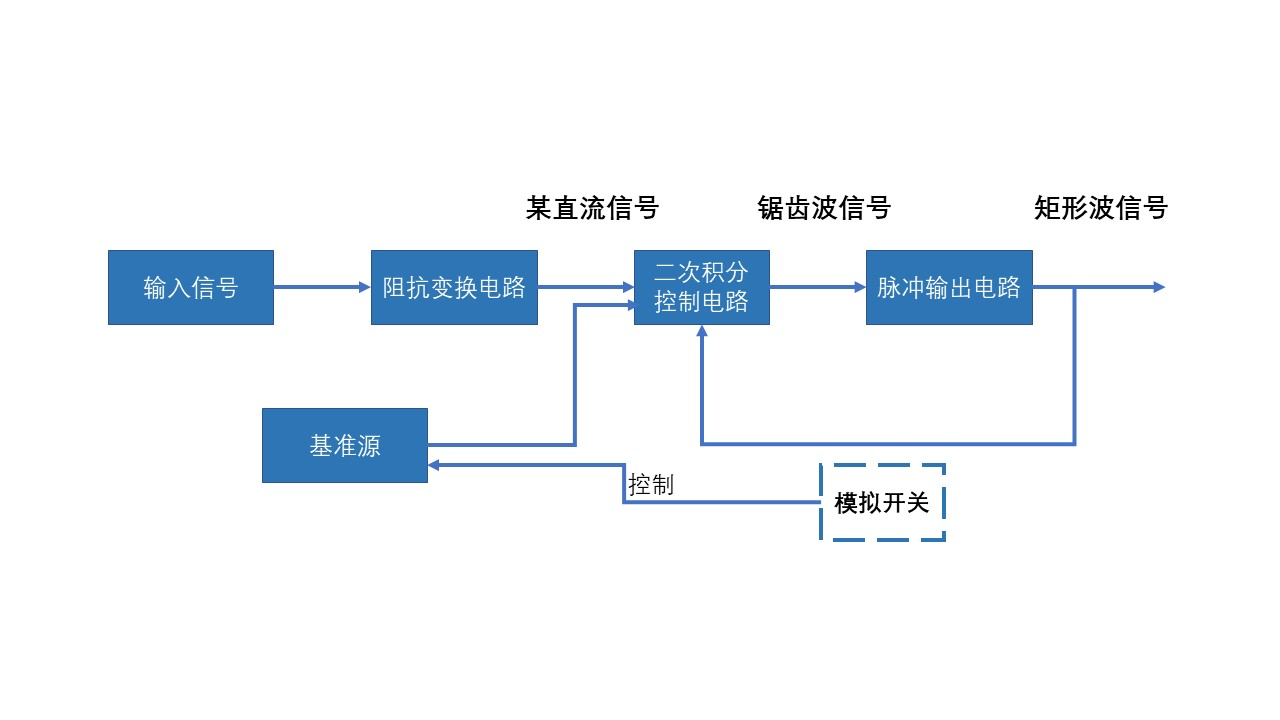
\includegraphics[width=1\textwidth]{fig/flow.jpg}
    \caption{线性V/F转换器电路原理框图}
    \label{fig:flow}
\end{figure}

\subsection{优缺点分析}

555单稳态、模拟开关(三极管)及集成运算放大器搭建的电路,实现的电压-频率转换在10K Hz范围内,能实现相当高的转换精度(大约在几赫兹左右,干扰过大除外),且器件均为常见的简易器件,电路搭建方便,易于操作和理解。在满足设计任务的条件下经济实惠,性价比高。

\section{模块设计}

线性V/F转换电路主要由积分电路、脉冲输出电路及反馈控制电路组成。

\subsubsection*{总电路设计}

通过阻抗变换获得相应的输入电压,并输入积分电路得到脉冲输出电路的电压控制信号(锯齿波),经由脉冲控制反馈中的三极管导通和关闭,实现通过基准源来调控积分时间的长短,进一步调控脉冲输出(矩形波)的电压控制信号(锯齿波),循环往复,形成振荡,实现电压到频率的线性转换。

\subsection{输入信号:电源分压电路}

电源电压为$12V$,电压输出范围为$0 \sim 10 V$,所以选择一个$R_1=2 K\Omega $的定值电阻与一个$10 K\Omega$的滑动变阻器$R_{w1}$串联,电压可调范围为$0 \sim 10 V$,符合指标要求。电路图如图\ref{fig:fig1}所示。

\begin{figure}[htbp]
    \centering
    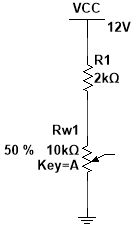
\includegraphics[width=0.2\textwidth]{fig/fig1.jpg}
    \caption{电源分压电路}
    \label{fig:fig1}
\end{figure}

\subsection{阻抗变换:电压跟随器电路}

共集电极电路的输入高阻抗、输出低阻抗特性,使得它在电路中可以起到阻抗匹配的作用,能够使得后一级的放大电路更好地工作。

电压跟随器输出电压近似等于输入电压幅度,并对前级电路呈高阻抗态,对后级电路呈低阻状态,因而对前后级电路起到“隔离”作用。基本原理还是利用它的输入阻抗高、输出阻抗低的特点。即输入电压不受后级电路阻抗影响。一个对前级电路相当于开路,输出电压又不受后级阻抗影响的电路当然具备隔离作用,及前后两级电路间互不影响。

为保证输入电压$0 \sim 10 V$不变,则必须保证其滑变的传入电路阻抗不变,加一个电压跟随器,可以使后续电路不影响滑变的阻抗,使输入电阻保持不变,反馈电路中接一电阻,使平衡输入端,提高跟随精度。电路图如\ref{fig:fig2}所示。

\begin{figure}[htbp]
    \centering
    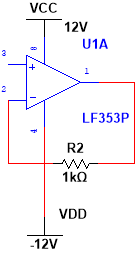
\includegraphics[width=0.2\textwidth]{fig/fig2.jpg}
    \caption{电压跟随器电路}
    \label{fig:fig2}
\end{figure}

\subsection{基准源}

使用一个$3V$的稳压管接入电路,即可提供一个$-3V$的稳定电压。选择$R_{10}=1K\Omega$的电阻保护稳压管。电路图如图\ref{fig:fig3}所示。

\begin{figure}[htbp]
    \centering
    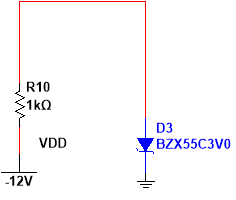
\includegraphics[width=0.3\textwidth]{fig/fig3.jpg}
    \caption{基准源电路}
    \label{fig:fig3}
\end{figure}


\subsection{积分电路}

利用集成运放可构成精度高、线性好的压控振荡器。积分电路输入电压变化的速率与输入电压的大小成正比,如果积分电容充电使输出电压达到一定程度后,使它迅速放电,然后输入电压再给它充电,如此循环往复,产生振荡,其振荡频率与输入电压成正比,即压控振荡器。

积分电路采用运放构成的反相积分电路,运放的同相端接入$10K\Omega$的失调电阻,反向端接入一个$5.1K\Omega$的电阻,然后再与$10K\Omega$滑变串接,保证其对称性,减小失调电流引起的误差。滑动变阻器可以调节输出锯齿波的周期,二极管起到保护运放的作用。电路图如图\ref{fig:fig4}所示。

\begin{figure}[htbp]
    \centering
    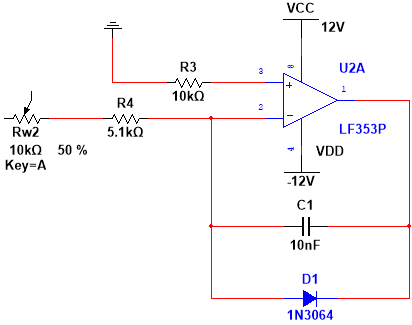
\includegraphics[width=0.4\textwidth]{fig/fig4.jpg}
    \caption{积分电路}
    \label{fig:fig4}
\end{figure}

\subsection{脉冲输出电路}

单稳态触发器只有一个稳定状态,一个暂稳态。在外加脉冲的作用下,单稳态触发器可以从一个稳定状态反转到一个暂稳态。由于电路中$RC$延时环节的作用,该暂态维持一段时间后又回到原来的稳态,暂稳态维持的时间取决于$RC$的参数值。

脉冲宽度$T_w = 1.1RC$,$R_7 = 3K\Omega$,$C_2 = 10nf$,由此计算得$T_w=32us$,此电路构成单稳态触发器,当积分电压经过0时触发单稳态($V_c \leqq  \frac{1}{3} V_{cc}$),输出宽度一定的脉冲去控制积分器。所以当$U_0 = 0V$时,单稳态触发电压:

\begin{equation}
V_c = \frac{1}{3} V_{cc} = \frac{R_5}{R_5 + R_6} = 4V
\end{equation}
则$R_5:R_6 = 1:2$,取$R_5=1K\Omega$,$R_6 = 2K\Omega$。电路图如图\ref{fig:fig5}所示。

\begin{figure}[htbp]
    \centering
    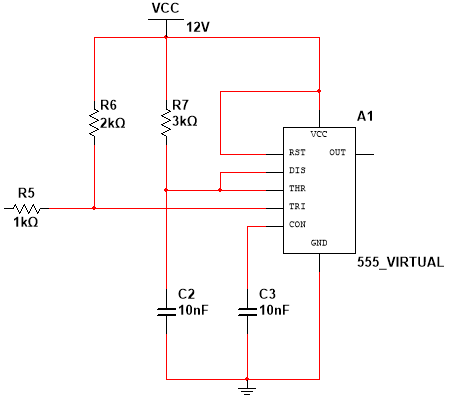
\includegraphics[width=0.4\textwidth]{fig/fig5.jpg}
    \caption{脉冲输出电路}
    \label{fig:fig5}
\end{figure}

\subsection{开关电路}

晶体三极管的实际开关特性决定与管子的工作状态。晶体三极管输出特性有三个工作区,即截止区、放大区、饱和区。

若要使晶体三极管工作于开关接通的状态,就应该使其工作与饱和区;要使晶体管工作于开关断开的状态,就应使之工作于截止区,发射级电流$i_e = 0$,此时晶体三极管处于截至状态,相当于开关断开。电路图如图\ref{fig:fig6}所示。

\begin{figure}[htbp]
    \centering
    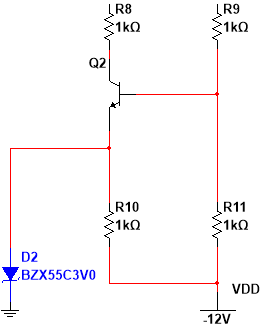
\includegraphics[width=0.3\textwidth]{fig/fig6.jpg}
    \caption{开关电路}
    \label{fig:fig6}
\end{figure}

积分电路先对基准源进行定时线性积分到一定电压高度$U_h$,触发脉冲输出F控制积分电路自动切换到对输入信号反向积分,到积分电压过零时积分控制电路又转换为对基准源积分。循环往复形成振荡,产生脉冲输出。

电路采用二次积分方法进行转换,当恒定宽度正脉冲输出时,信号反馈到输入端控制开关闭合。此时积分器对$-U_r$进行正向积分,而积分电压$U_c$的高度$U_h$与基准电压以及重放电常数有关。一旦输出脉冲消失,开关S截至,积分器对$U_i$反向积分直到过零。

\subsection{相关参数计算}

由设计任务分析得到,$R_8$与$R_9$是偏置电阻,其必须满足当脉冲输出电路为低电平(即为“0”)时,三极管不导通,即是b和e电位差小于管压降$0.7V$,$V_e=-3V$,则$V_b$的取值小于$-2.3V$,所以:
\begin{equation}
V_b = -  \frac{R_8}{R_8+R_9} * V_{cc}
\end{equation}
取$R_8 = R_9 = 1K\Omega$,则此时:
\begin{equation}
V_b = -  \frac{R_8}{R_8+R_9} * V_{cc} = -6V < -2.3V
\end{equation}
满足条件,脉冲输出电路输出电压为高电平(即为“1”)时,此时满足:
\begin{equation*}
    \begin{cases}
        V_b>-2.3V \\
        V_b = \frac{R_8}{R_8+R_9} * (V_{cc} + V_i) = -1V > -2.3V
    \end{cases}
\end{equation*}
进而可以可以通过一定输出宽度的脉冲控制积分器的积分动作。

对于$R_{10}$的选取,为了防止流入稳压管的电流过大,接入一个限流电阻,取$R_{10}=1K\Omega$。

滑动变阻器$R_{w2}$主要调节整个电路的周期,对脉冲宽度影响很小;电阻$R_7$主要决定脉冲宽度。

考虑到流过稳压管的电流范围,三极管基极电阻$R_9=1 K\omega$时满足要求。

为了保护运算放大器,在反向积分电路中加入二极管,使积分输出端为0时反向截止。

如果三角波幅值未达到要求,可以通过调节三极管集电极的电阻来控制产生的三角波幅值。

\subsection{总电路图}

经过上述分析,在multisim中搭建仿真电路如图\ref{fig:Circuitdiagram}所示。
\begin{figure}[htbp]
    \centering
    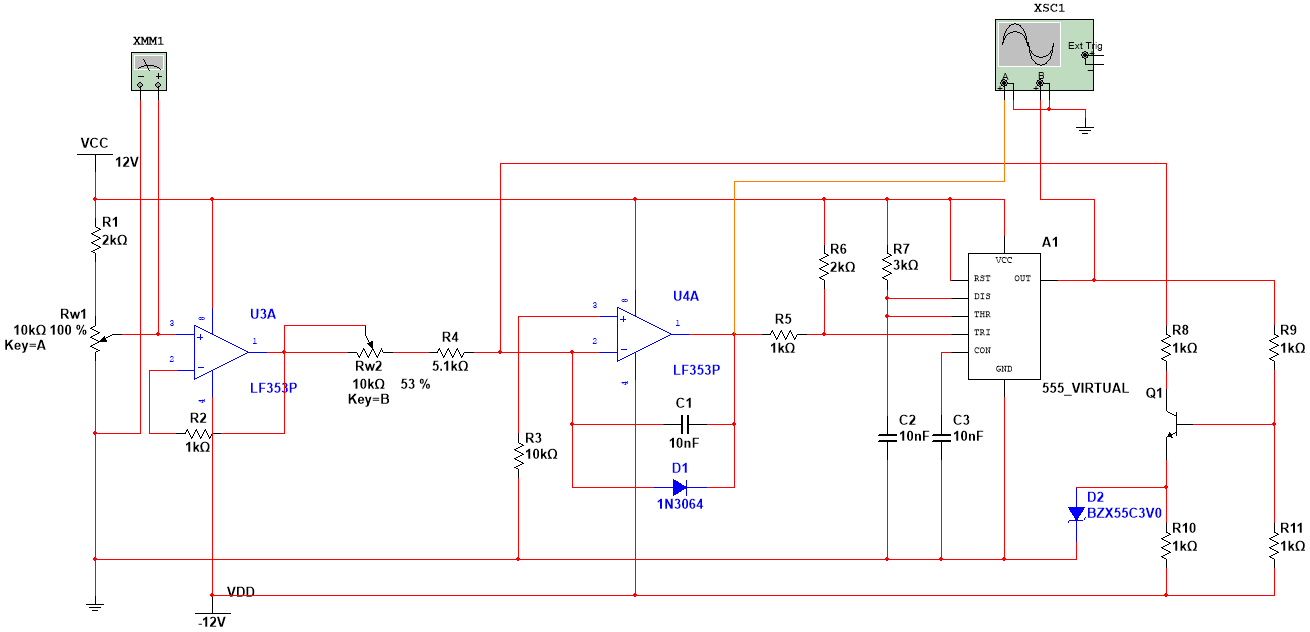
\includegraphics[width=1\textwidth]{fig/Circuit_diagram.jpg}
    \caption{线性V/F转换器仿真电路图}
    \label{fig:Circuitdiagram}
\end{figure}

\section{计算机软件仿真}

在multisim中进行仿真调试,利用示波器观察电路的实际输出波形,仿真波形如图\ref{fig:Simulated_waveform}所示。

\begin{figure}[htbp]
    \centering
    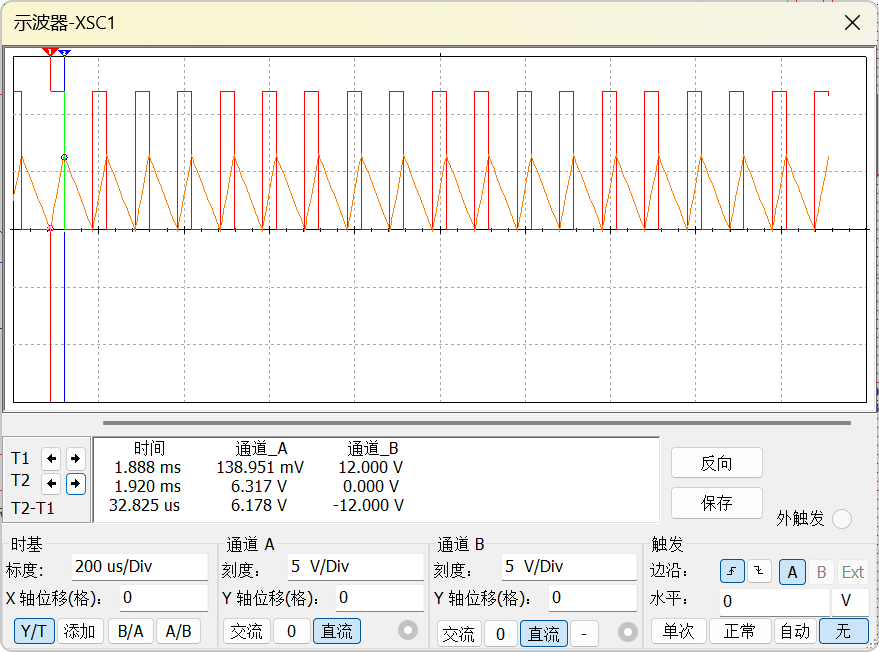
\includegraphics[width=0.8\textwidth]{fig/Simulated_waveform.jpg}
    \caption{线性V/F转换器仿真波形图}
    \label{fig:Simulated_waveform}
\end{figure}

从图中可以看出,输出波形为矩形波,且脉宽为32.825 $\mu s$,满足设计要求。

\section{实际组装与调试}

线下课程中,在实验室的实际硬件平台上利用给出硬件搭建电路,进行调试,通过示波器观察电路的实际输出波形。

实验所用元器件如表\ref{tab:components}所示。

\begin{longtable}[htbp]{ccc}
    \caption{元器件清单}\\
    \label{tab:components}\\
    \toprule
    元件名称       & 元件型号     & 数量 \\
    \midrule
    \endfirsthead
    
    \multicolumn{3}{c}{续表~\thetable\hskip1em 元器件清单}\\
    \toprule
    元件名称       & 元件型号     & 数量 \\
    \midrule
    \endhead
    
    \bottomrule
    \multicolumn{3}{r}{\small 续下页}
    \endfoot
    
    \bottomrule
    \endlastfoot
    
    集成运算放大器 & LF353P       & 2    \\
    三极管         & S9013        & 1    \\
    二极管         & 1N3064       & 1    \\
    稳压管         & BZX55C3V0    & 1    \\
    电阻           & 1K$\Omega$   & 6    \\
    电阻           & 2K$\Omega$   & 2    \\
    电阻           & 3K$\Omega$   & 1    \\
    电阻           & 5.1K$\Omega$ & 1    \\
    电阻           & 10K$\Omega$  & 1    \\
    滑动变阻器     & 10K$\Omega$  & 2    \\
    电容           & 0.1$\mu$F    & 3    \\
\end{longtable}

实际搭建电路图如图\ref{fig:Real_circuit}所示。

\begin{figure}[H]
    \centering
    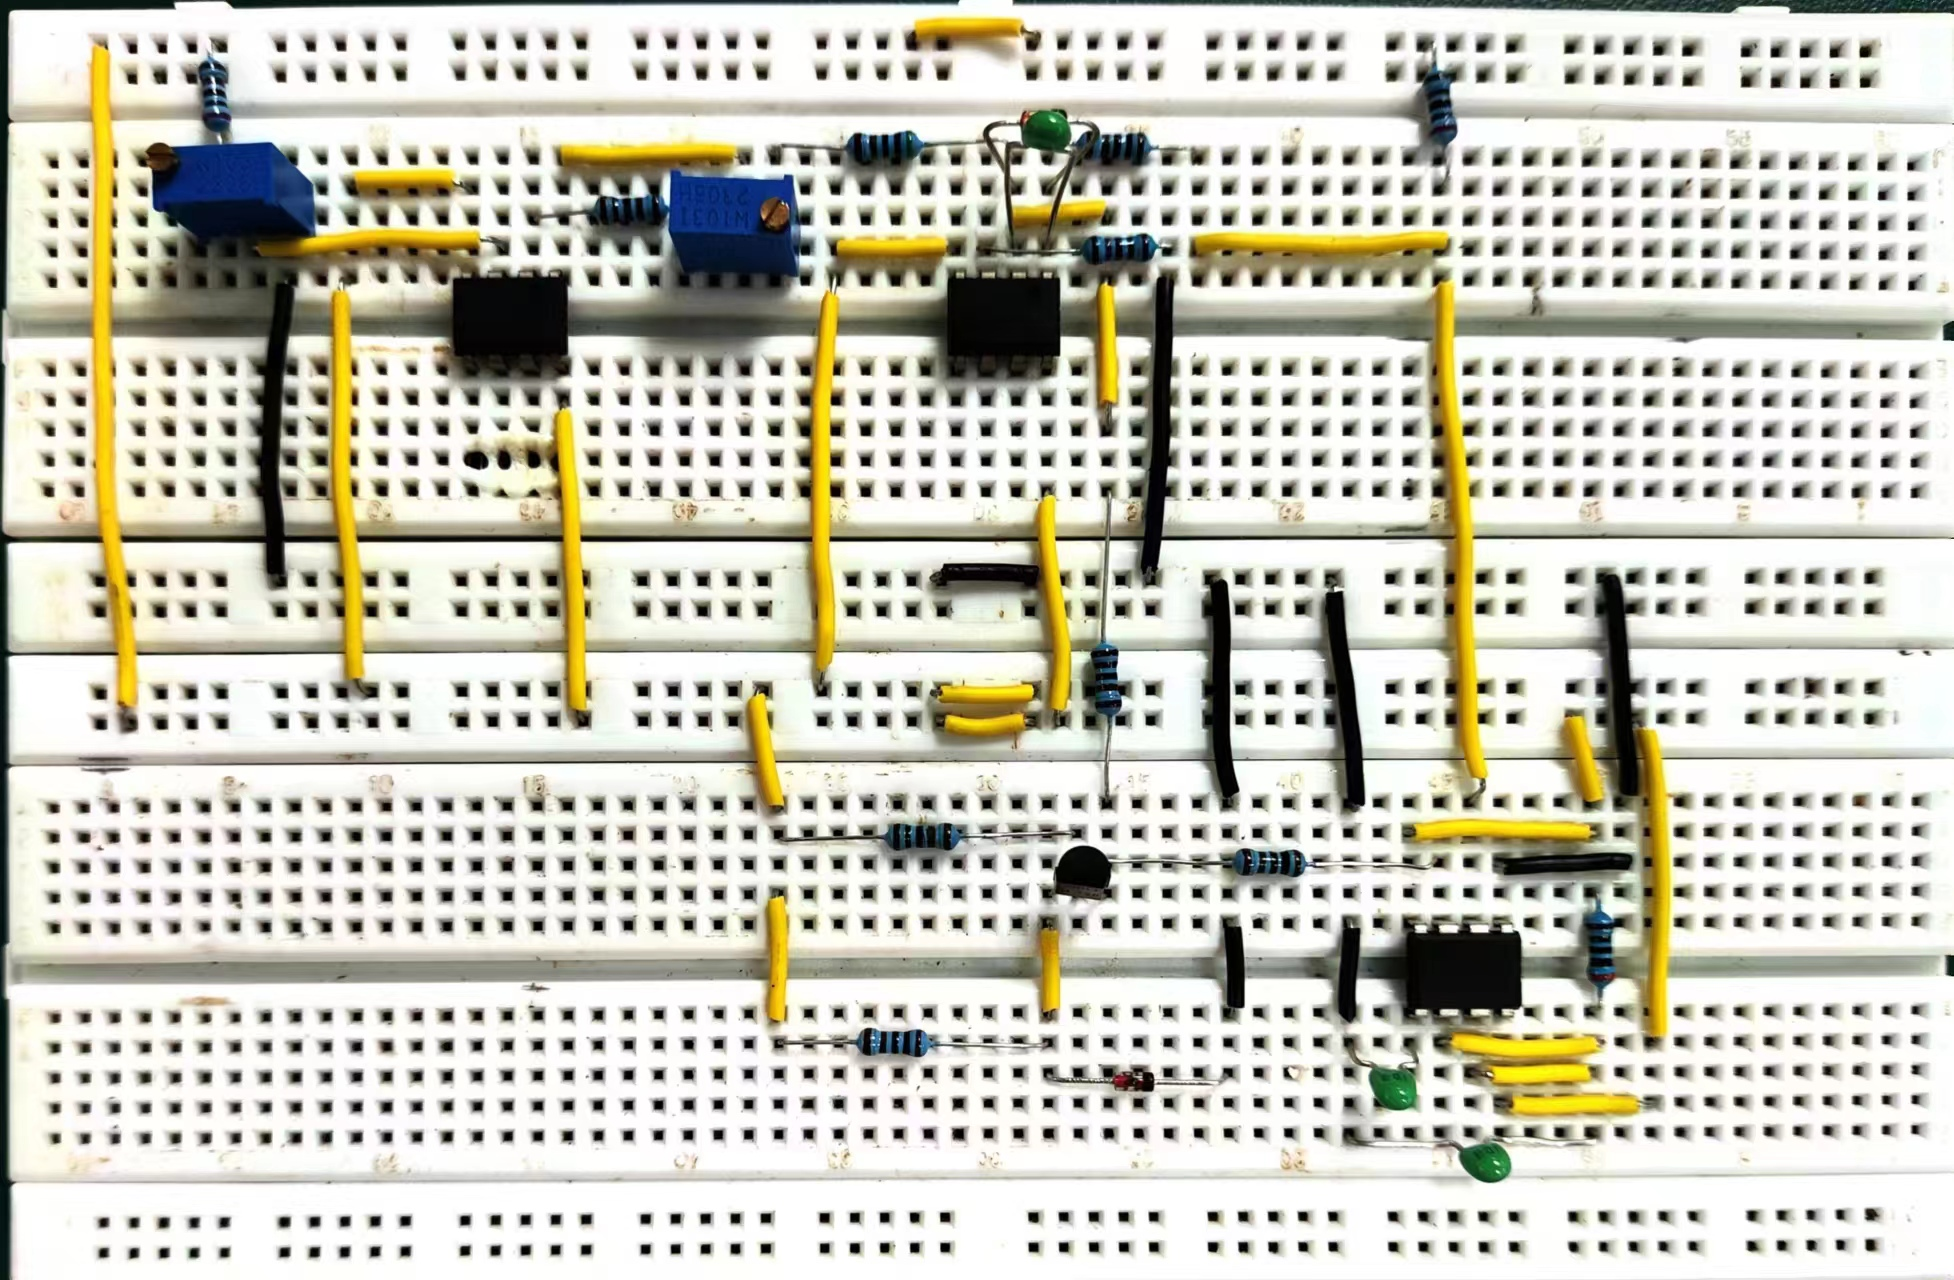
\includegraphics[width=0.8\textwidth]{fig/Real_circuit.jpg}
    \caption{线性V/F转换器实际搭建电路图}
    \label{fig:Real_circuit}
\end{figure}

\newpage
利用示波器测量相关数据,其中输入信号为$5V$、$10V$的正弦波,输出信号为$5$K Hz、$10$K Hz的矩形波,测量结果如图\ref{fig:Real_waveform}所示。

\begin{figure}[htbp]
    \centering
    \begin{minipage}[t]{0.48\textwidth}
        \centering
        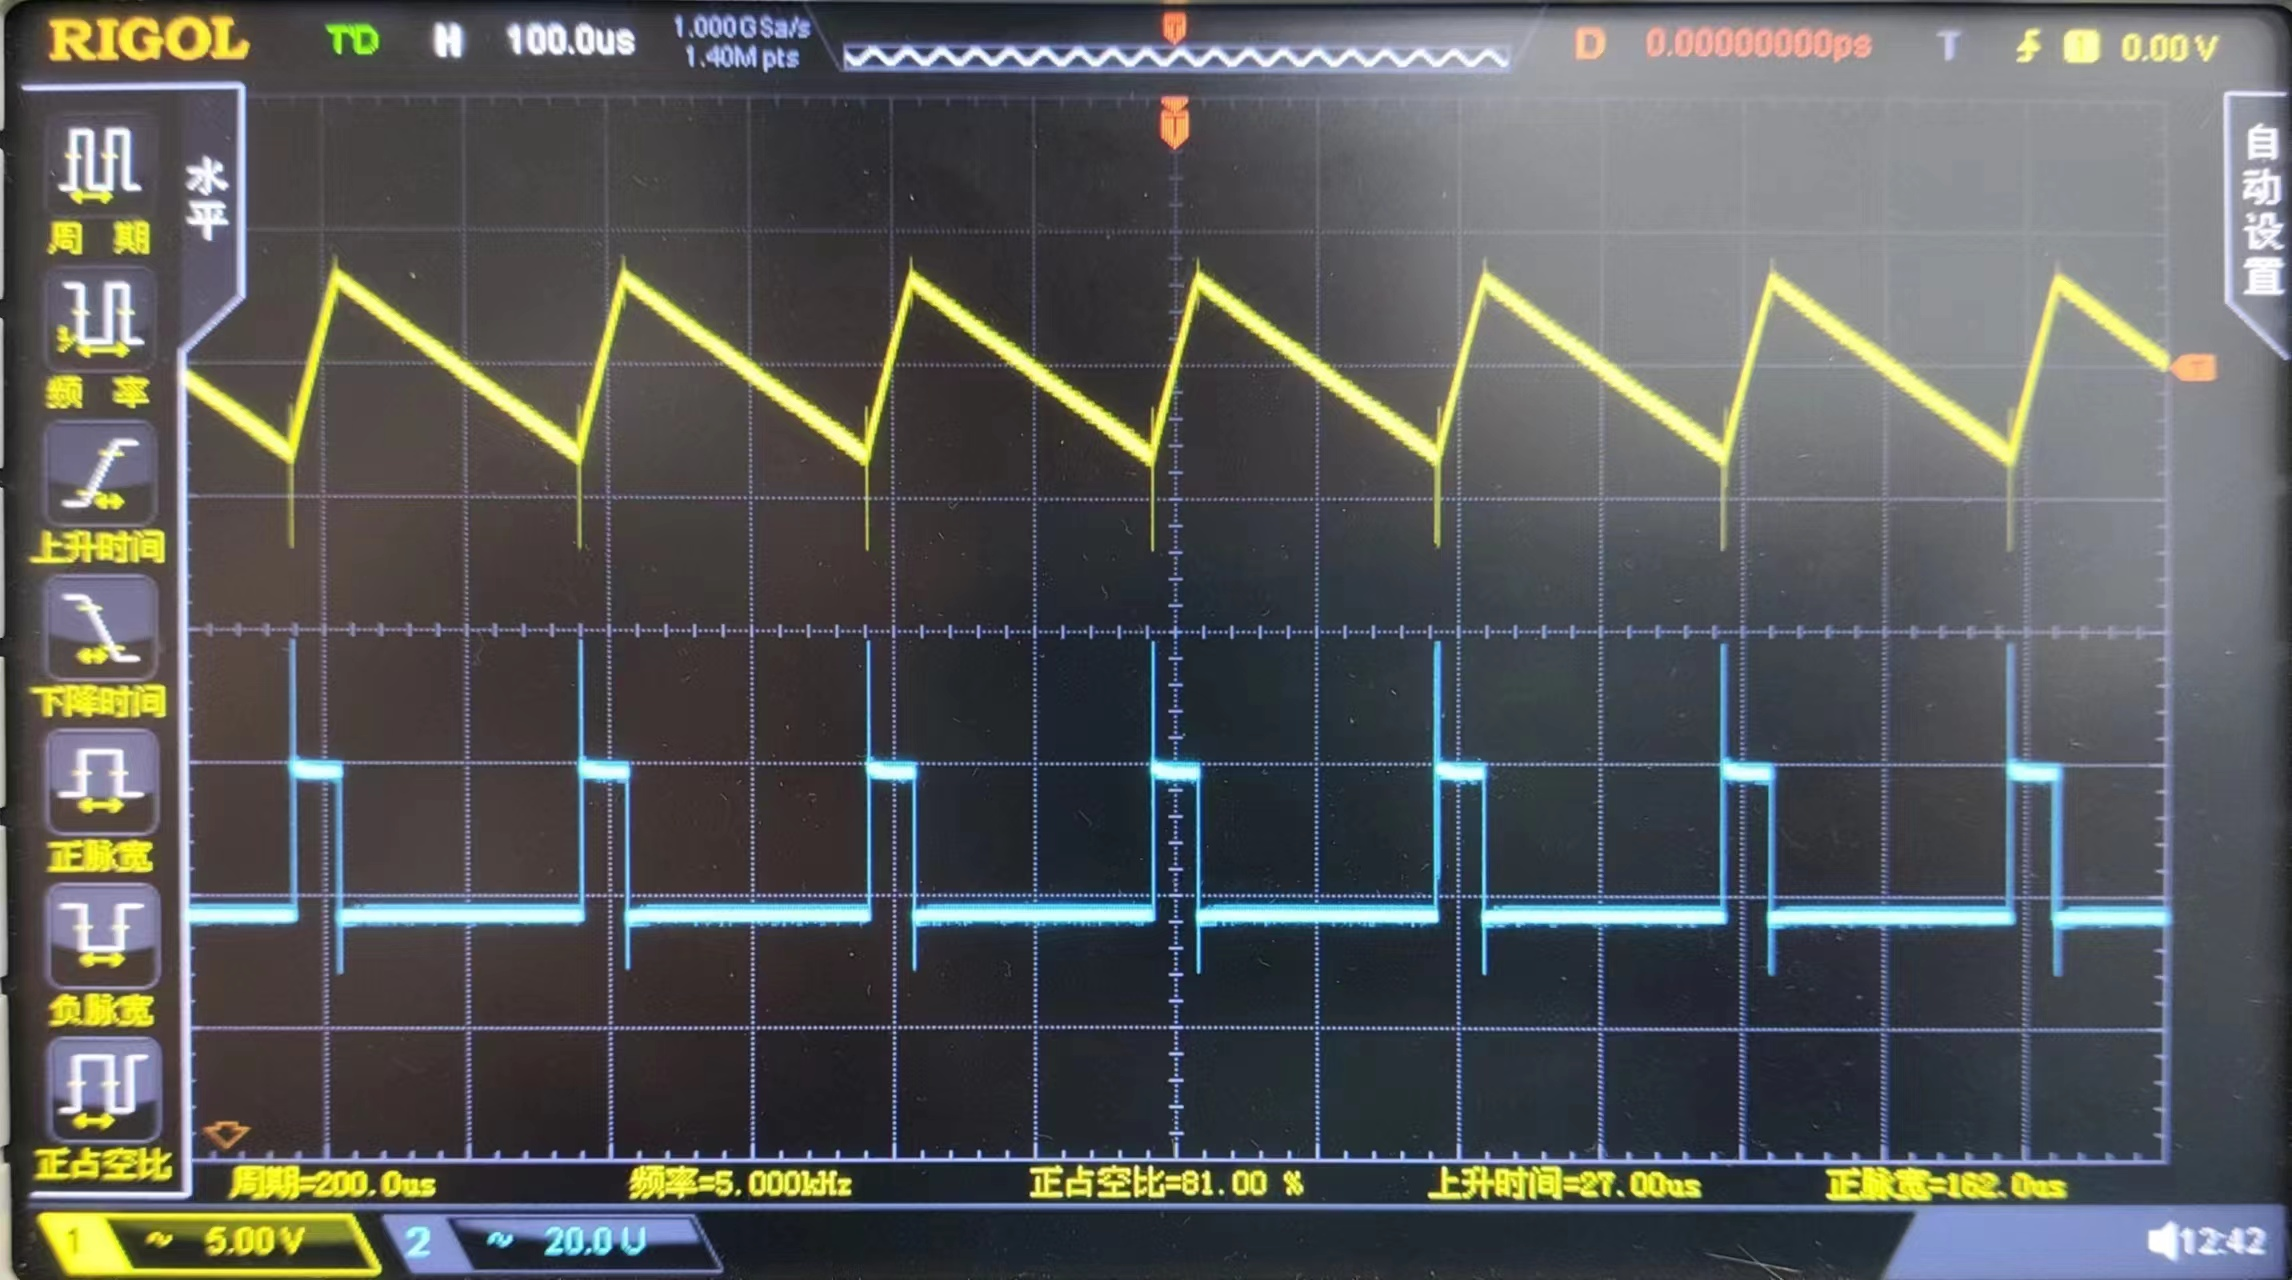
\includegraphics[width=\textwidth]{fig/5V.jpg}
        \caption*{输入信号5V}
    \end{minipage}
    \hfill
    \begin{minipage}[t]{0.48\textwidth}
        \centering
        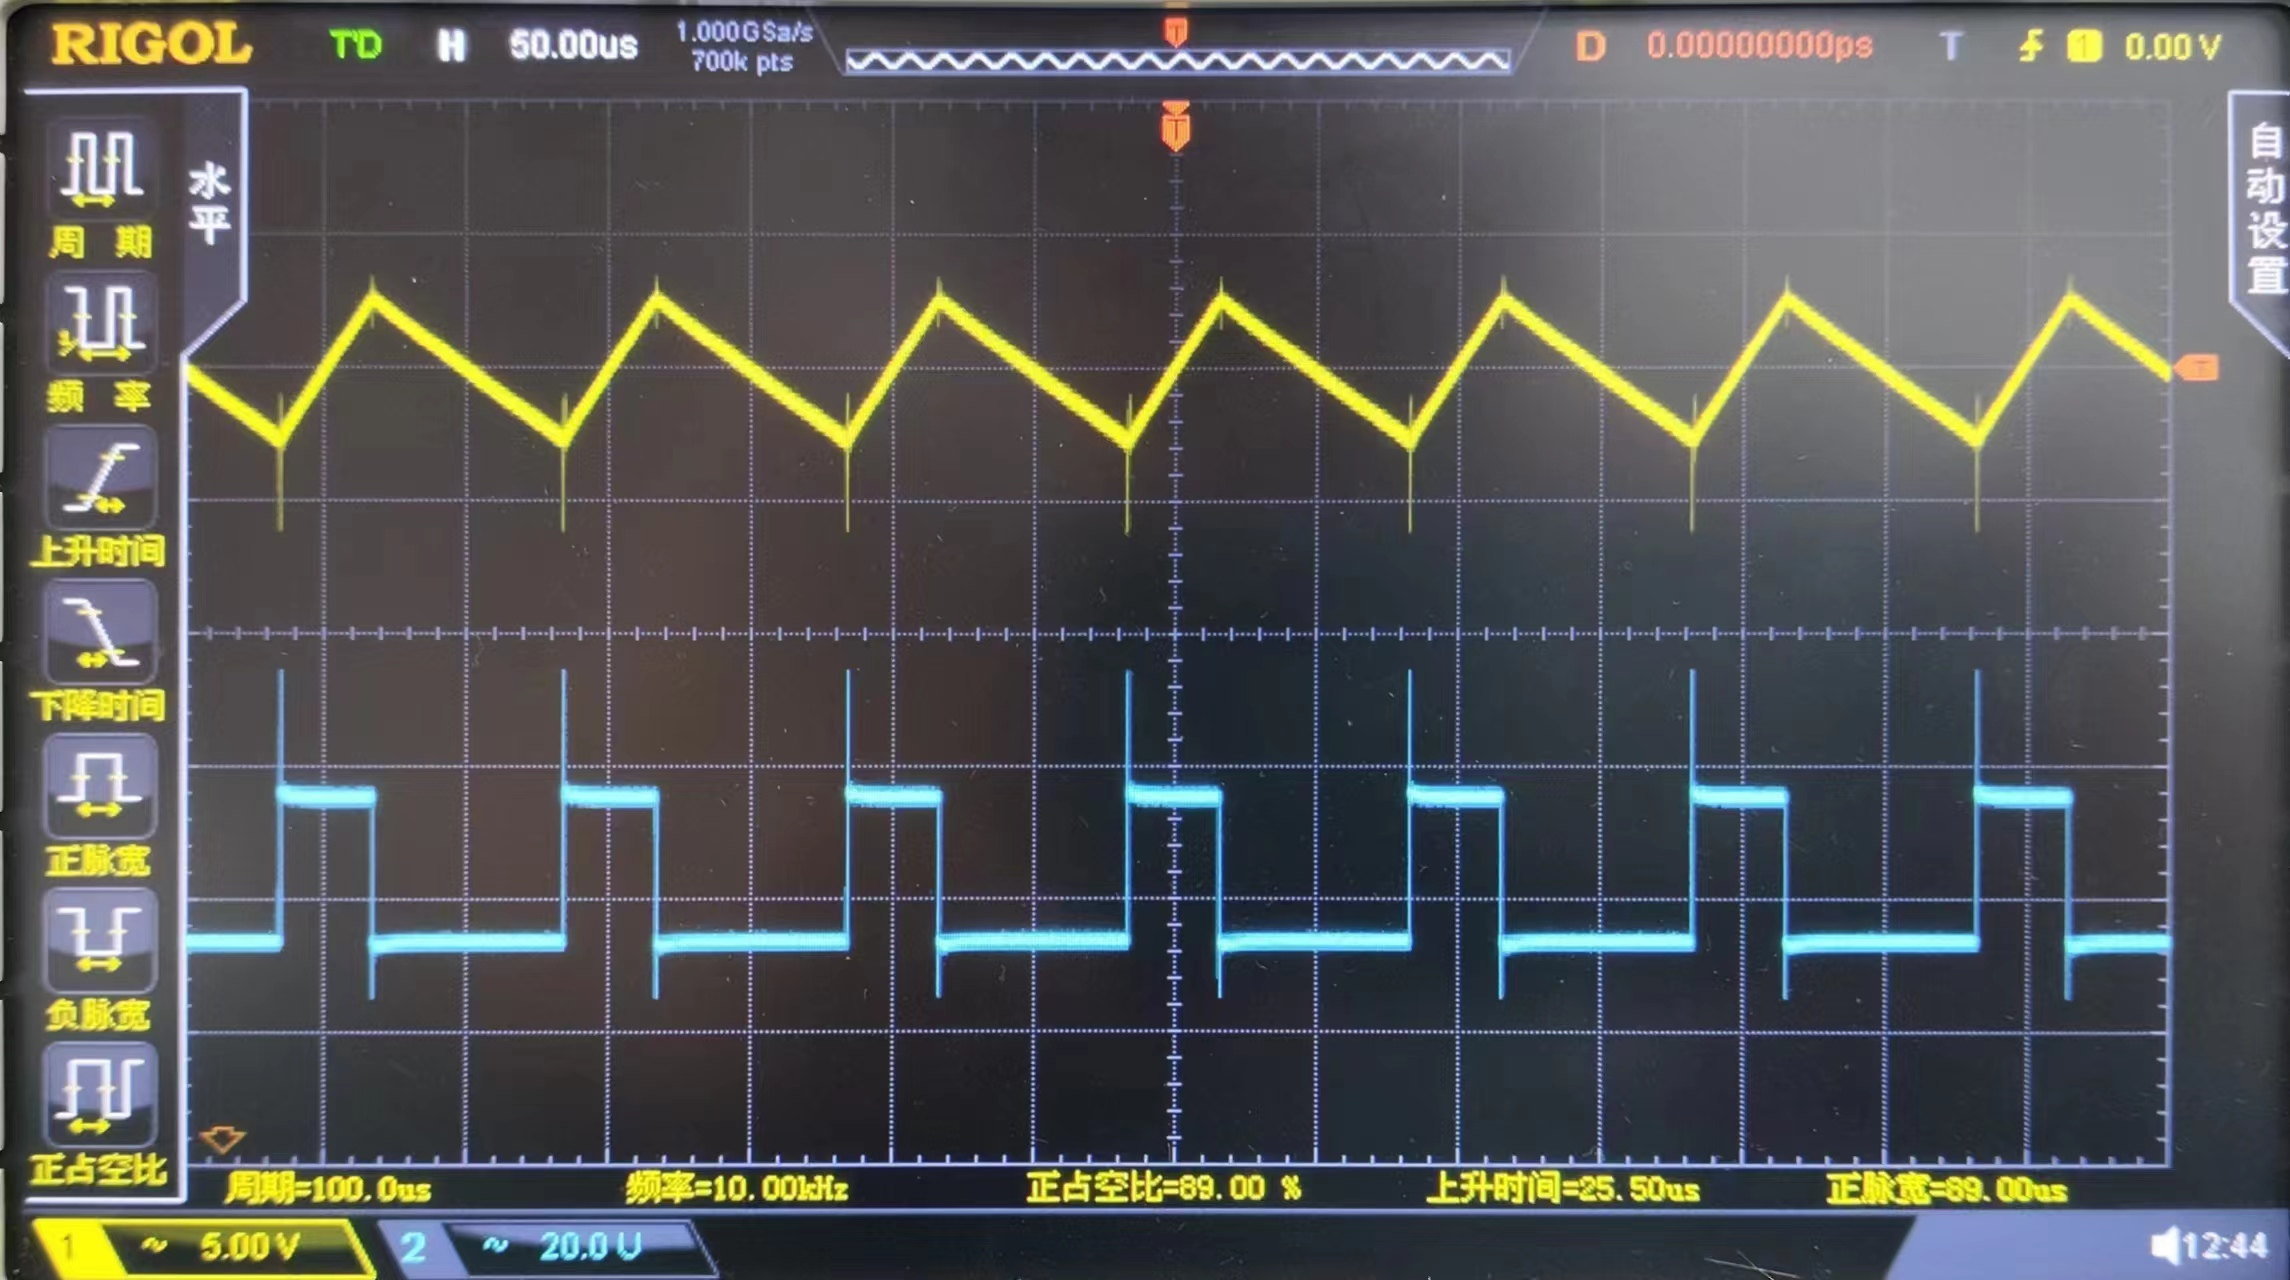
\includegraphics[width=\textwidth]{fig/10V.jpg}
        \caption*{输入信号10V}
    \end{minipage}
    \caption{不同输入信号下的输出波形}
    \label{fig:Real_waveform}
\end{figure}

\section{数据分析及改进}

搭建实际电路,通过示波器测量不同输入信号下的输出频率,结果如表\ref{tab:frequency}所示。

\begin{table}[htbp]
    \centering
    \caption{不同输入信号下的输出频率}
    \label{tab:frequency}
    \begin{tabular}{|c|c|c|c|c|c|}
        \hline
        电压/V & \makecell{理想输出\\频率/K Hz} & \makecell{实际输出\\频率1/K Hz} & \makecell{实际输出\\频率2/K Hz} & \makecell{平均输出\\频率/K Hz} & 误差值/Hz \\
        \hline
        1       & 1.000    & 1.000     & 1.004     & 1.002    & 2      \\
        2       & 2.000    & 1.998     & 2.008     & 2.003    & 3      \\
        3       & 3.000    & 3.000     & 3.004     & 3.002    & 2      \\
        4       & 4.000    & 4.004     & 4.012     & 4.008    & 8      \\
        5       & 5.000    & 5.006     & 5.014     & 5.010    & 10     \\
        6       & 6.000    & 6.008     & 6.016     & 6.012    & 12     \\
        7       & 7.000    & 7.010     & 7.016     & 7.013    & 13     \\
        8       & 8.000    & 8.012     & 8.018     & 8.015    & 15     \\
        9       & 9.000    & 9.014     & 9.020     & 9.017    & 17     \\
        10      & 10.00    & 10.00     & 10.00     & 10.00    & 0      \\
        \hline
    \end{tabular}
\end{table}

绘制实际输出频率与输入电压的关系曲线如图\ref{fig:linear_relationship}所示,两曲线基本重合,表明实际搭建的电路工作良好。

\begin{figure}[htbp]
    \centering
    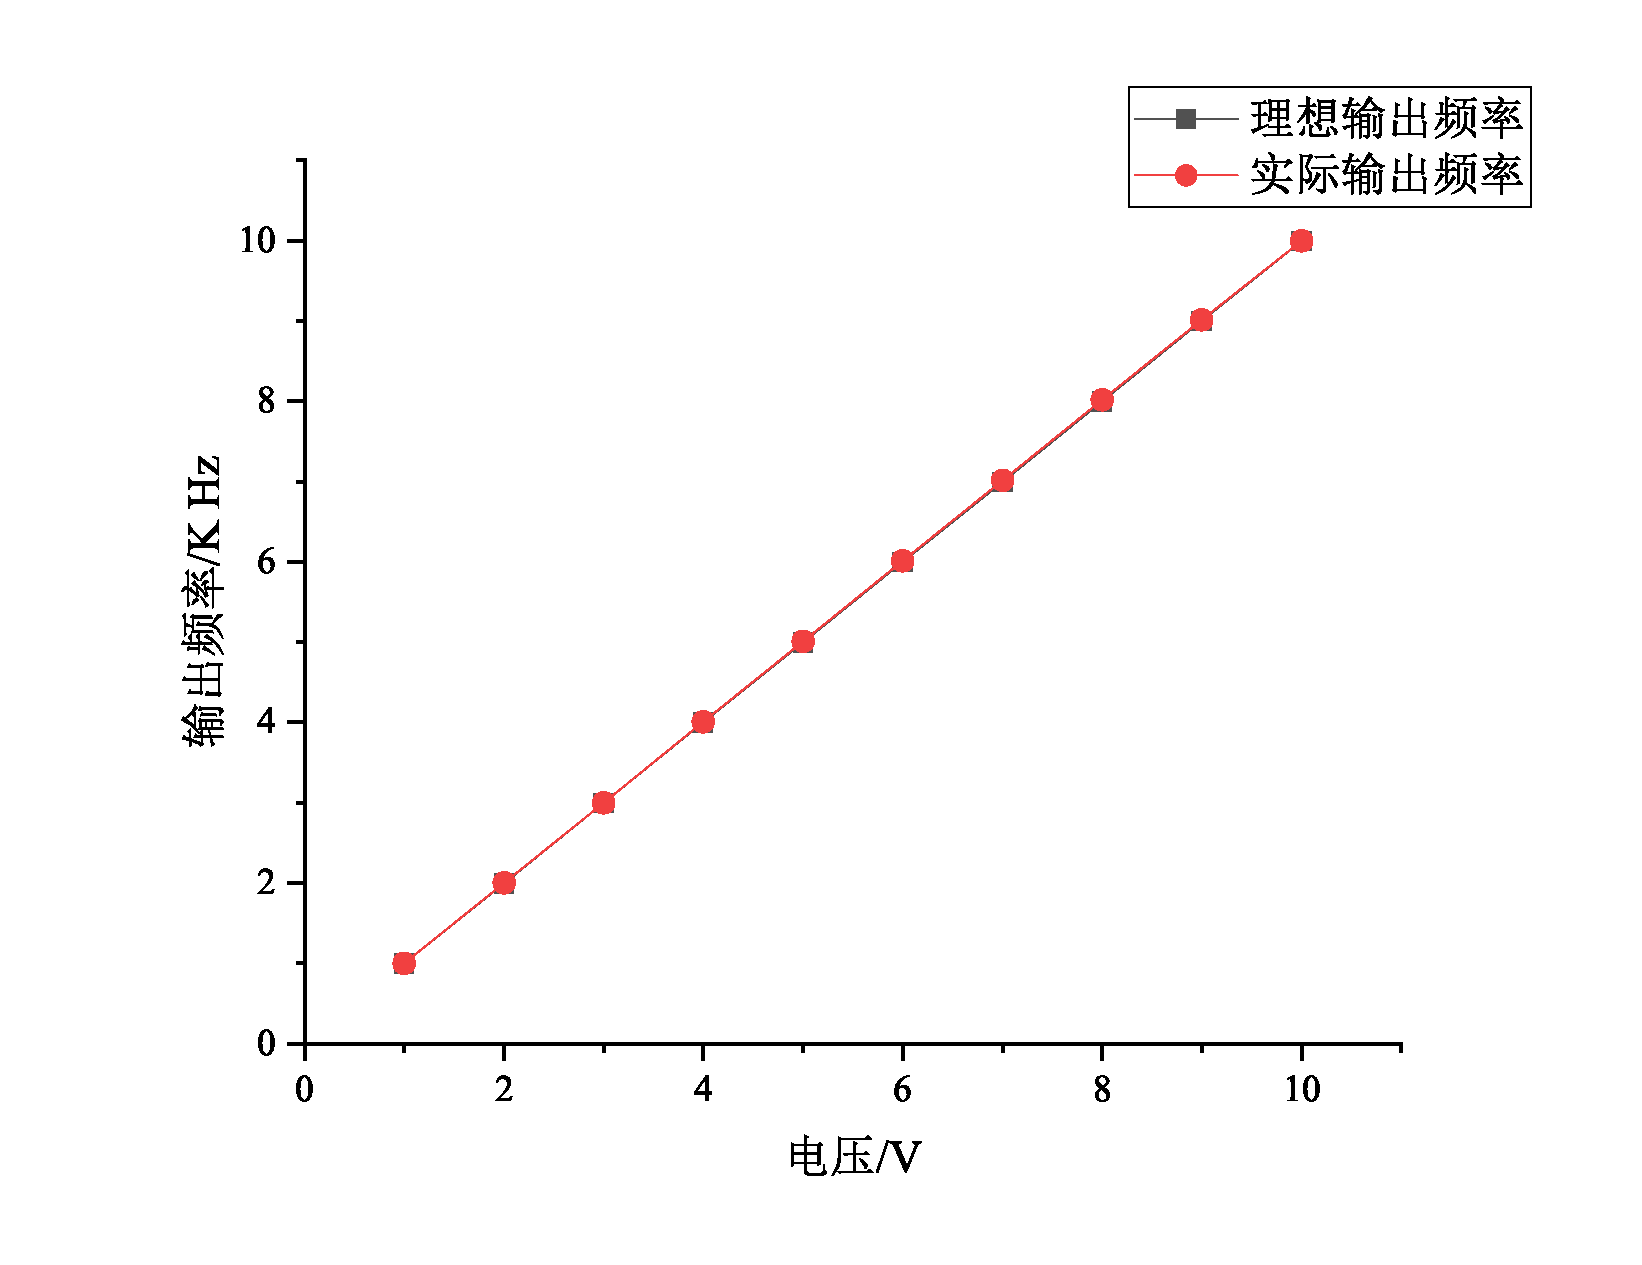
\includegraphics[width=0.8\textwidth]{fig/linear_relationship.eps}
    \caption{实际输出频率与输入电压的关系曲线}
    \label{fig:linear_relationship}
\end{figure}

实际测得输出频率误差在$\pm 30$ Hz以内,满足设计要求。

\newpage
\subsubsection*{改进方法}

从上述实验数据可以看出所设计的电路精度基本符合要求。若想继续改进,提高电路精度,可采取如下方法:

\begin{itemize}
    \item 在不同的输入电压的条件下,精确调节失调电阻$R_{w2}$,使得误差进一步减小;
    \item 对整个电路的相关参数进行更加细致的微调。
    \item 在电源正负极、NE555P单稳态触发器8号引脚与地之间接入较大的电容,减少噪音的干扰。
\end{itemize}

\section{心得与体会}

在电路设计过程中,我学会了熟练操作multisim等仿真软件,掌握了基本的电路设计方法,对电路的基本原理有了更深的理解。在仿真过程中,我遇到了一些小问题,诸如元件的查找、仿真测量工具的使用等,我通过在网络上查找资料等方式,独立地、顺利地解决了所有问题,并得到了满意的结果。

实际搭建电路时,由于不太熟悉面包板、一些原件的使用,导致第一次连接完毕后没有得到正确的结果。在课后我研究了面包板的使用、查找了相关元件的引脚图,仔细检查了电路的连接,最终成功地搭建了正确的电路,得到了波形。经过调整,测得了比较满意的数据。在测量数据时,由于不会使用示波器,造成了一些小困扰。后来通过向同学请教,最后得以完成本实验。

本次课程设计带给我的收获不小,综合了模拟电子技术课程知识,而在搭接电路时,也让我发现自己需要更细心和耐心,在本专业学习中,这两点也尤为重要。比如连接电路时最好分块采用不同颜色的线,而且要尽量使线路简洁明了,在帮同学检查电路时,很多缠绕复杂、交叉、跨接的线路让我看得很烦恼,而往往连接复杂的线路也容易把自己绕晕,因此连接电路时细节可谓是关键的。

与此同时,与同学和老师之间的交流也让我受益良多,当我面对问题毫无头绪的时候,交流带给我新的思路,在此非常感谢帮助过我的老师和同学。通过这次实验,我看到了自己的不足,提高了我的动手能力和独立思考,查阅资料,交流合作等方面的能力,也让我学到了很多课本里学不到的东西,细心可以减少很多不必要的麻烦,也唯有静下心来,才能找到问题的所在。

\newpage
\nocite{*}
\bibliographystyle{plain}
\begin{thebibliography}{99}

    \bibitem{ref1}童诗白, 华成英. 《模拟电子技术基础(第五版)》. 高等教育出版社, 2015.
    \bibitem{ref2}杨上河. 《电子技术实验与模拟电子技术课程设计》. 西安电子科技大学出版社. 2012.09.

\end{thebibliography}

\newpage
\section*{附录}

\begin{figure}[htbp]
    \centering
    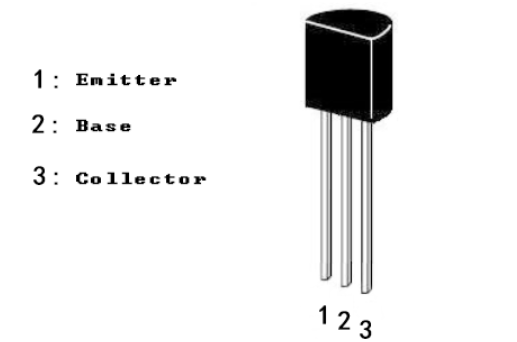
\includegraphics[width=0.6\textwidth]{fig/S9013.png}
    \caption{S9013三极管引脚图}
    \label{fig:S9013}
\end{figure}

\begin{figure}[htbp]
    \centering
    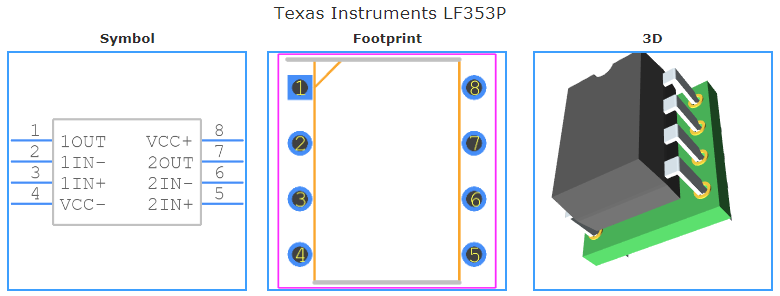
\includegraphics[width=0.6\textwidth]{fig/LF353P.png}
    \caption{LF353P集成运放引脚图}
    \label{fig:LF353P}
\end{figure}

\begin{figure}[htbp]
    \centering
    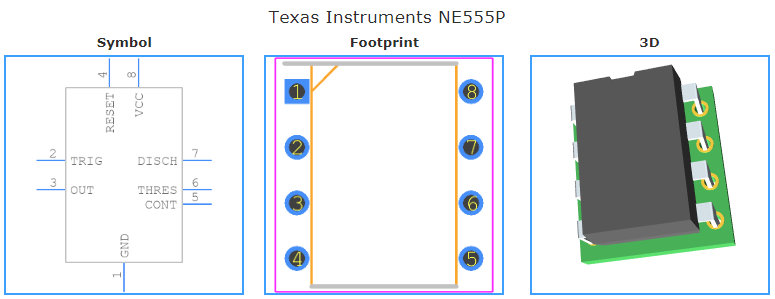
\includegraphics[width=0.6\textwidth]{fig/NE555P.png}
    \caption{NE555P单稳态触发器引脚图}
    \label{fig:NE555P}
\end{figure}

\end{document}
